\documentclass[10pt]{standalone}
\usepackage{tikz}
\usetikzlibrary{
  calc,
  patterns,
  decorations.pathmorphing,
}





\begin{document}

\noindent
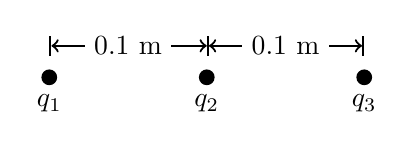
\begin{tikzpicture}
  

  \fill (-2,0) circle (0.1) node[below=0.1cm] {$q_1$};
  \fill (0,0) circle (0.1) node[below=0.1cm] {$q_2$};
  \fill (2,0) circle (0.1) node[below=0.1cm] {$q_3$};
  \draw[|<->, thick] (-2,0.4) -- ++(2,0) node[midway, fill=white] {0.1 m};
  \draw[|<->|, thick] (0,0.4) -- ++(2,0) node[midway, fill=white] {0.1 m};




\end{tikzpicture}




\end{document}